\documentclass[t,pdflatex]{beamer}
\usepackage[utf8]{inputenc}

\usetheme{Frankfurt}

\title{Learning Breakout using NEAT}
\author{James~T.~Murphy~III\thanks{\url{jamesmurphy@math.utexas.edu}}\and{}Skyler~Thomas\thanks{\url{skylerthomas0@gmail.com}}}
\institute{The University of Texas at Austin}
\date\today

\begin{document}
\section{Title}

    \begin{frame}

        \titlepage

    \end{frame}

\section{Introduction}
    \begin{frame}

        In 2015 youtuber SethBling trained a neural network to play and successfully beat, the first level of Super Mario World.
        \frametitle{A neat application of a neat algorthim}
        \begin{figure}
            \centering
            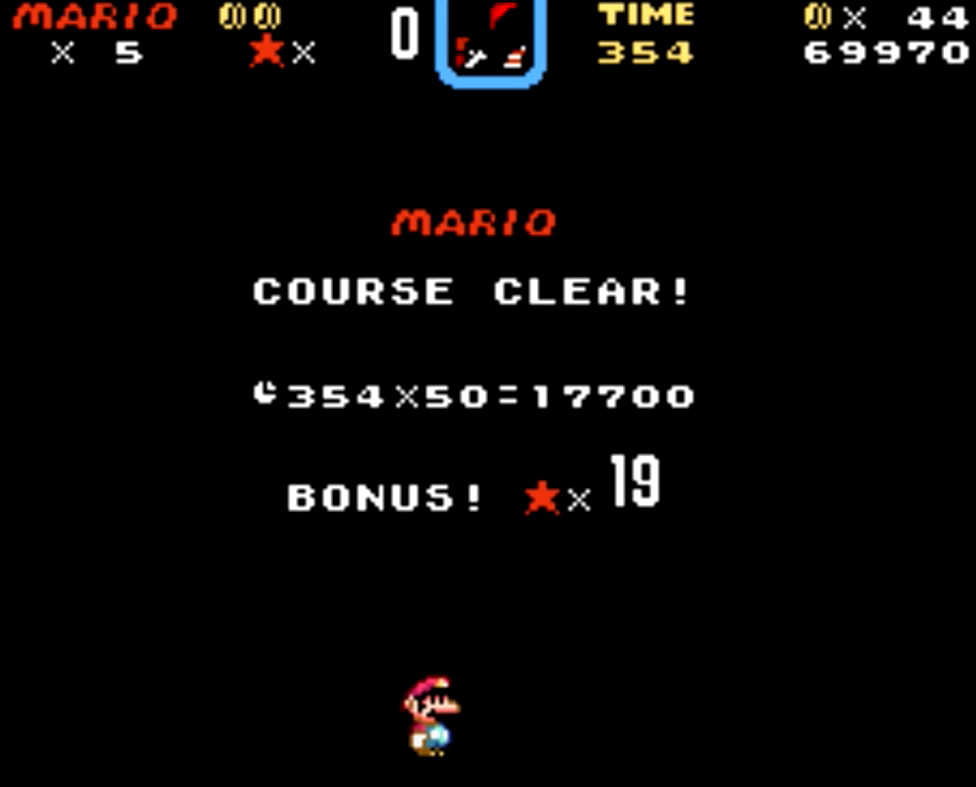
\includegraphics[width=.54 \textwidth]{mario.png}
        \end{figure}

    \end{frame}

    \begin{frame}

        \frametitle{How}
        This was done using the Neural Evolution of Augmenting Technologies AlgOrithm (NEAT-O) from the 2002 paper by Stanley and Mikkulainen.



    \end{frame}

    \begin{frame}

        \frametitle{\texttt{NEAT}, the algorithm}
        \begin{enumerate}[1]
            \item \texttt{NEAT} is a type of genetic algorithm that follows the biological metaheuristics of fitness begets evolution.

        \end{enumerate}

    \end{frame}

        \begin{frame}

        \frametitle{Breakout}
        \begin{itemize}
            \item In the game, a layer of bricks lines. A ball travels across the screen, bouncing off the top and side walls of the screen. When a brick is hit, the ball bounces away and the brick is destroyed. The player loses a turn when the ball touches the bottom of the screen. To prevent this from happening, the player has a movable paddle to bounce the ball upward, keeping it in play.
        \end{itemize}


    \end{frame}

\section{Experiment}

    \begin{frame}

        \frametitle{Null Hypothesis & Experiment}
        \begin{itemize}
            \item Null Hypothesis: NEAT will learn something.
            \item Experiment: A copy of \texttt{NEAT} was made using the python pygame package and a \texttt{NEAT} network was made using then python NEAT package.

        \end{itemize}

    \end{frame}

\section{Results}

    \begin{frame}

        \frametitle{Results}
        Qualitatively, it appears there are three eras
        \begin{enumerate}
            \item Pre-ball-tracking arc: The network does nothing or makes small and arbitrary movements
            \item Ball-tracking arc: It is apparent the ball is tracking the ball, but there are cases the network hasn't learned to do deal with yet.
            \item Aiming-arc: The network actively moves to and aims the ball to clear all 520 blocks.
        \end{enumerate}

    \end{frame}


    \begin{frame}

        \frametitle{Results}
         \begin{figure}[h!]
            \centering
            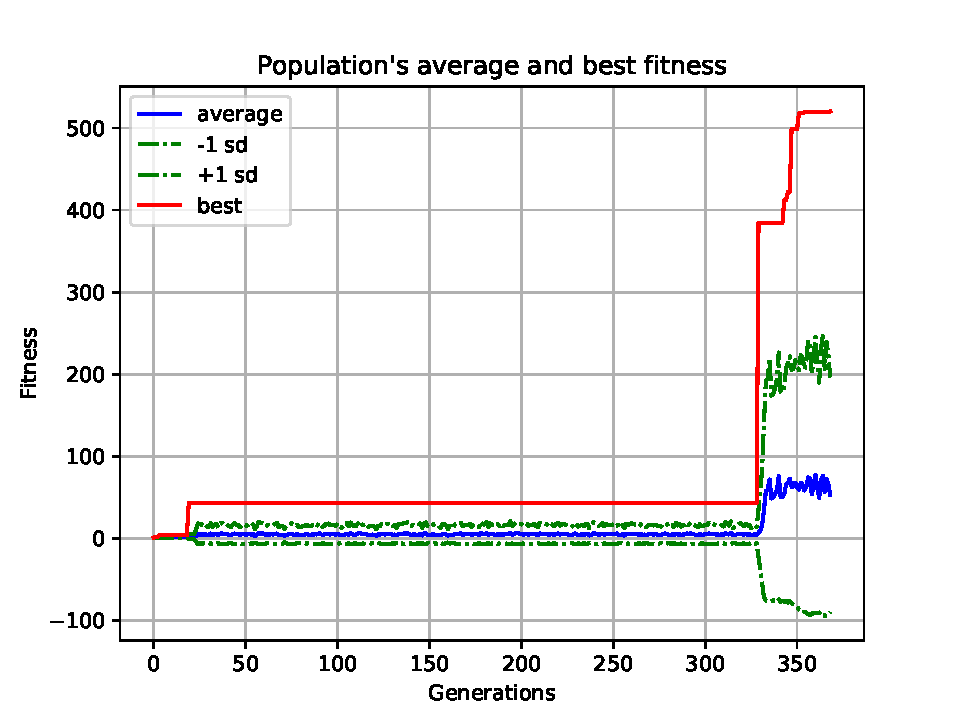
\includegraphics[width=.54 \textwidth]{avg_fitness.pdf}
            \caption{\textit{A successful training experiment.} In this case, the pre-ball-tracking era lasts
                until around generation 325, where the network abruptly learns how to track the ball.
                The ball-tracking era then lasts until around generation 350, where the network learns to avoid missing stray blocks. The aiming era is reached in the last few generations.
                Generations of 200 individuals took an average time of 2.835 sec to evaluate on an
                Intel Core i7-4790K @ 4.00GHz in parallel on 6 cores. Total runtime $\approx$ 17.5 minutes.}
        \end{figure}

    \end{frame}

\section{Discussion}

        \begin{frame}

        \frametitle{Discussion}
         \begin{itemize}
             \item It is difficult to predict what the network will and will not learn with respect to the inputs to the network and more so with respect to the hyperparameters.
             \item The network is incredibly sensitive to parameters and hyperparameters
             \item The number of generations required to successfully complete the task has a critical point.
         \end{itemize}

    \end{frame}

        \begin{frame}

        \frametitle{Future}
        \begin{itemize}
            \item Explore the relationship between fitness and and solution
            \item Compare with DQN



    \end{frame}


\end{document}
